\documentclass[tikz,11pt]{standalone}
% --- Typography ---
\usepackage[sc,osf]{mathpazo} % Palatino with small caps & oldstyle figures
\usepackage{microtype}
% --- TikZ libraries ---
\usetikzlibrary{arrows.meta,positioning,calc,shadows}
% --- TikZ styles ---
\definecolor{pewblue}{RGB}{31,119,180}
\definecolor{pewgray}{RGB}{90,90,90}
\tikzset{
  >=Latex,
  box/.style={
    rectangle, rounded corners=3pt,
    draw=pewgray!70, line width=0.9pt,
    fill=white, drop shadow,
    align=left, inner sep=7.5pt, text width=4.5cm
  },
  arrow/.style={->, line width=1.1pt, draw=pewblue},
}
\begin{document}
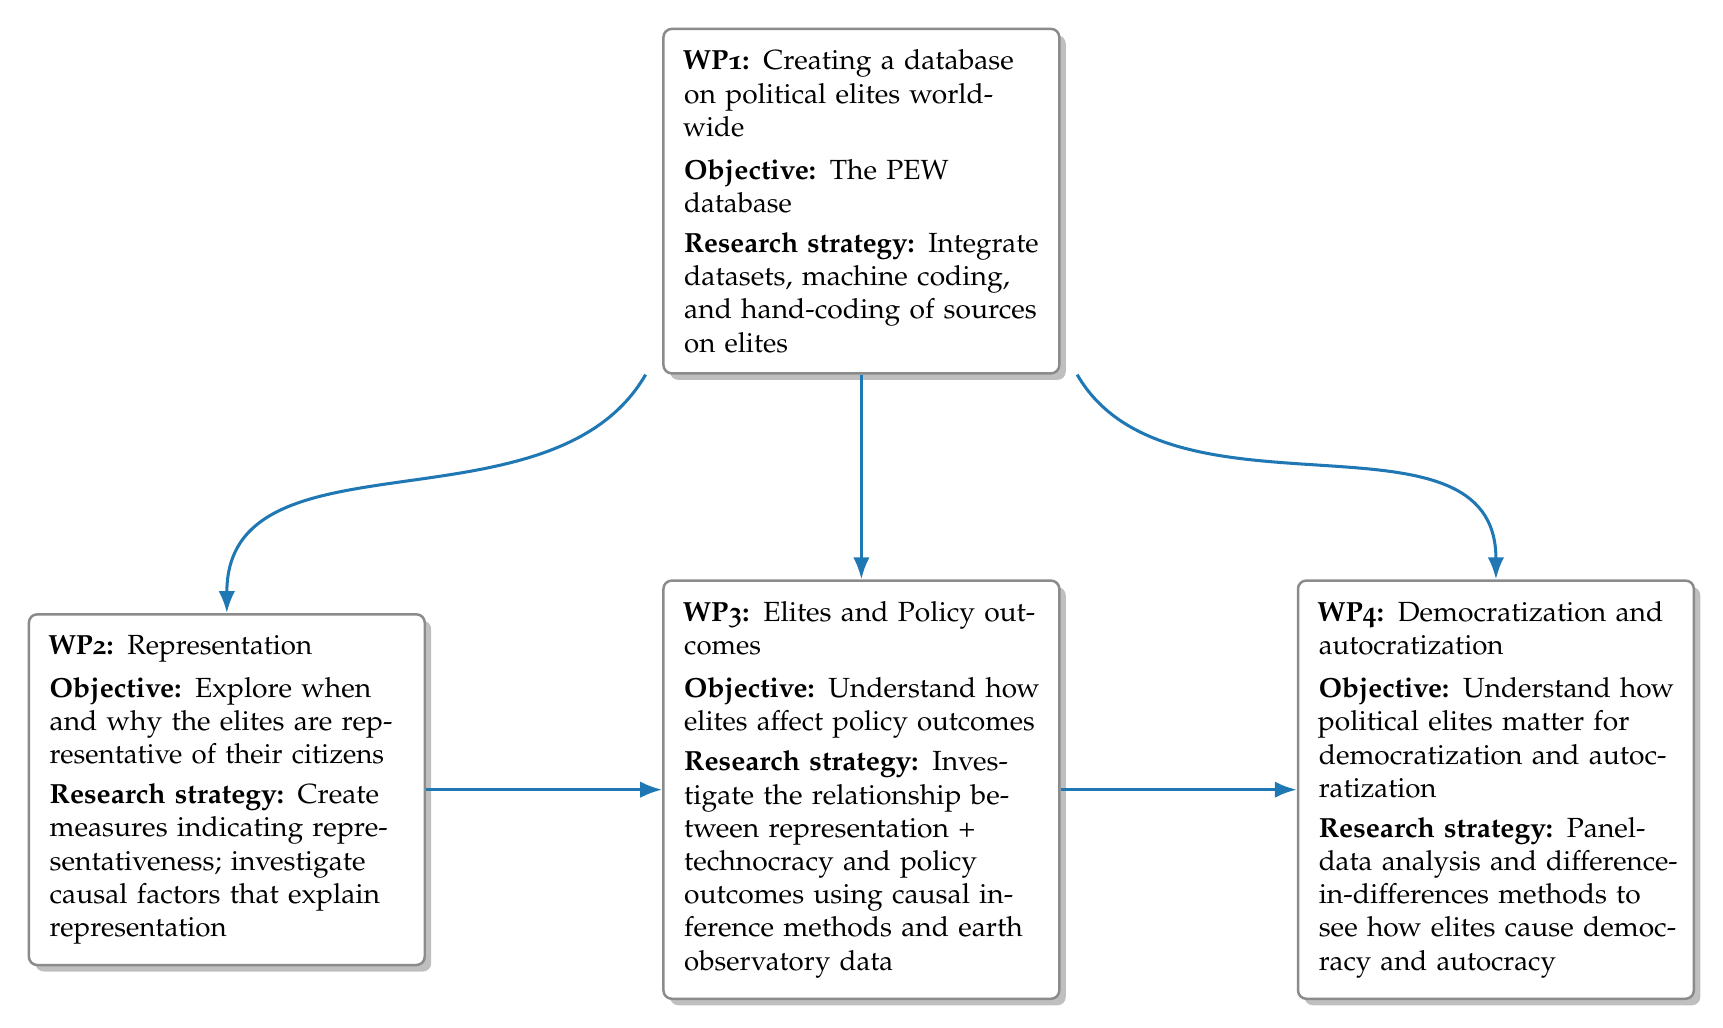
\begin{tikzpicture}[node distance=2.2cm]
% --- Nodes ---
\node[box] (wp1) {
  \textbf{WP1:} Creating a database on political elites worldwide\\[0.35em]
  \textbf{Objective:} The PEW database\\[0.25em]
  \textbf{Research strategy:} Integrate datasets, machine coding, and hand-coding of sources on elites
};
\node[box, below=2.6cm of wp1] (wp3) {
  \textbf{WP3:} Elites and Policy outcomes\\[0.35em]
  \textbf{Objective:} Understand how elites affect policy outcomes\\[0.25em]
  \textbf{Research strategy:} Investigate the relationship between representation + technocracy and policy outcomes using causal inference methods and earth observatory data
};
\node[box, left=3cm of wp3] (wp2) {
  \textbf{WP2:} Representation\\[0.35em]
  \textbf{Objective:} Explore when and why the elites are representative of their citizens\\[0.25em]
  \textbf{Research strategy:} Create measures indicating representativeness; investigate causal factors that explain representation
};
\node[box, right=3cm of wp3] (wp4) {
  \textbf{WP4:} Democratization and autocratization\\[0.35em]
  \textbf{Objective:} Understand how political elites matter for democratization and autocratization\\[0.25em]
  \textbf{Research strategy:} Panel-data analysis and difference-in-differences methods to see how elites cause democracy and autocracy
};
% --- Arrows ---
\draw[arrow] (wp1) -- (wp3);                                  % down
\draw[arrow] (wp2) -- (wp3);                                  % left -> center
\draw[arrow] (wp3) -- (wp4);                                  % center -> right
% gentle, elegant diagonal links from WP1
\draw[arrow] ([xshift=-6pt]wp1.south west) to[out=240,in=90] (wp2.north);
\draw[arrow] ([xshift=+6pt]wp1.south east) to[out=300,in=90] (wp4.north);
\end{tikzpicture}
\end{document}